\documentclass{mcmthesis}
\mcmsetup{%CTeX = false,                       %% ʹÓà CTeX Ì×װʱ£¬ÉèÖÃΪ true
        tcn = 2312787, problem = D,             %% tcn is team control number
        sheet = true, titleinsheet = true,    %% sheet stands for summary sheet
        titlepage = false, abstract = true}    %% titlepage represents abstract page, true or false

%\usepackage{palatino}   %%COMAP¹Ù·½°æÎï×ÖÌå
%\usepackage{times}      %%ÂÞÂí×ÖÌ壬ֻ¶ÔÕýÎÄÆð×÷ÓÃ
\usepackage{txfonts}     %%Êýѧ¹«Ê½ÂÞÂí×ÖÌ壬¶Ô¹«Ê½ºÍÕýÎĶ¼Æð×÷ÓÃ



\title{\LaTeX{} Template for MCM/ICM }
\author{\team}
\date{\today}
\begin{document}

\begin{summary}
The 2014 Ebola virus (EBOV) outbreak in West Africa is so far the largest and
deadliest recorded in history. It is thus crucial to better understand the spread
of infection and to mitigate the outbreak in the affected countries.

We describe the epidemic using a delayed SEIQR
(susceptible-exposed-infective-quarantined-removed) model.
We fit the model to the most recent reported data of infected cases and deaths in Sierra Leone and Liberia.
To aid in planning for additional disease-control efforts,
we introduce Ebola treatment units (ETU) and pulse vaccination in this model.
We find that the EBOV epidemic begins to decrease and eventually end if people with Ebola
virus can be isolated in ETUs with medical care.

Based on the SEIQR model, we cluster the affected areas with Self-Organizing Map (SOM) neural network.
We then formulate a multi-layer dynamic drug distribution model incorporating the results of the SOM
clustering, which contributes significantly in controlling epidemic areas with
relatively high degree of urgency. With the goals of minimizing the
transportation cost and decreasing the unsatisfied demand for the urgency
logistics network, we employ the artificial immune system (AIS) to locate the
distribution center.chinatex

The main advantage of our approach is that the models utilize clever
algorithm allowing us to see clearly how preventions and interventions can
mitigate and eventually stop the epidemic. A limitation of our approach is
that we constrict the population flow within countries and underlie national
epidemic transmission. Results of our models not only support the
construction of a medical material delivery system, but also demonstrate the
needs for more ETUs to be established, supplied, and staffed.

\noindent
\textbf{Key Words:}
SEIQR Model; Self-Organizing Maps; Immune Algorithm; Deliver System;

\end{summary}


\maketitle



%\newpage
%\thispagestyle{empty}
%\begin{center}
%\bfseries\Large
%Synopsis/Memo/Handout
%\end{center}
%
%This is Synopsis/Memo/Handout.




\thispagestyle{empty}
\newpage
\tableofcontents
\newpage
\setcounter{page}{1}
\section{Introduction}

\subsection{Background}


The United Nations (UN) \cite{fonseca2020mapping} has set 17 Sustainable Development Goals (SDGs) that, if realized, would result in substantial enhancements to the quality of life for people worldwide. Implementation and achievement of this universal agenda will require well-designed development policies and partnerships with multiple stakeholders. Yet, these objectives are interrelated\cite{singh2018rapid}, and development in one area may have positive or negative repercussions on the others. 

Hence, reaching all 17 SDGs is a dynamic and difficult process that requires balancing competing national and international goals, budget constraints, and the effects of global crises such as technology developments, pandemics, climate change, regional conflicts, and refugee displacement\cite{shulla2021effects}. 
In this study, we examine the interwoven and multifaceted nature of the SDGs, as well as the obstacles and opportunities involved with achieving them. 

\subsection{Restatement of problems}


\begin{itemize}
\item minimizes the discomfort to the hands, or
\end{itemize}
We focus exclusively on the second definition.

\begin{itemize}
\item the initial velocity and rotation of the ball,
\end{itemize}

\begin{itemize}
\item the angular velocity of the bat,
\end{itemize}

\emph{center of percussion} [Brody 1986],



%=======
\begin{Theorem} \label{thm:latex}
\LaTeX
\end{Theorem}

\begin{Lemma} \label{thm:tex}
\TeX .
\end{Lemma}

\begin{proof}
The proof of theorem.
\end{proof}


\subsection{Other Assumptions}
D. E. Knuth \cite{Knuth},
the author of \textit{the Art of Computer Programming},
is a very famous computer scientist,
now living at Stanford University.




\section{Analysis of the Problem}

%LaTeX²åͼָÄÏ
\begin{figure}[ht]
\label{fig:aa}
\small
\centering
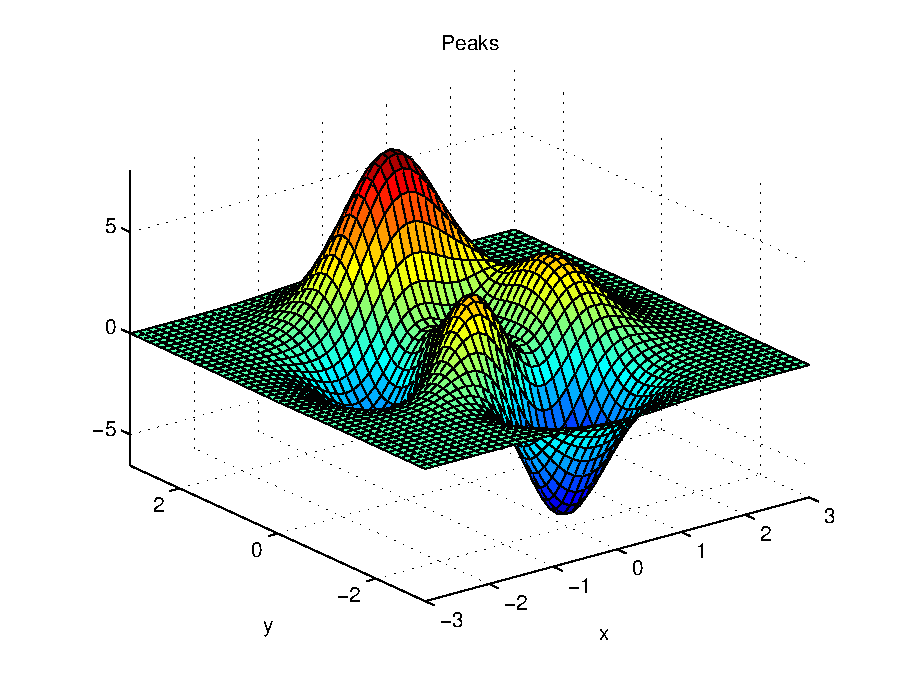
\includegraphics[width=12cm]{mcmthesis-aaa.eps}
\caption{The Curve Plane of System}
\end{figure}

%1£¬²»ÒªÓÃ×Óͼ£¬subfig£¬subfigure¡£
%2£¬¾¡Á¿¼õÉÙ¸¡¶¯»·¾³£¬Í¼¾¡Á¿£¬ËõСͼµÄռλ

It follows that
\begin{equation}\label{aa}
a^2 + b^2 = c^2
\end{equation}


The equation \eqref{aa} has told that

\[
\begin{pmatrix}
  a_{11}  & a_{12}  & a_{13}   \\
  a_{21}  & a_{22}  & a_{23}   \\
  a_{31}  & a_{32}  & a_{33}
\end{pmatrix}
= \frac{{Opposite}}{{Hypotenuse}}\cos^{-1} \theta \arcsin \theta
\]

\[
p_{j}=
\begin{cases}
0,             & \text{if $j$ is odd}\\
r!\,(-1)^{j/2},& \text{if $j$ is even}
\end{cases}
\]



\[
\arcsin \theta  = \oint\limits_\varphi \lim_{x \to \infty } \frac{n!}{r! (n - r)!} \eqno (23)
\]


\section{ Data structure construction }
\subsection{ Literature review }
\subsubsection{ Relationships between SDGs }
We provide a summary of recent research contributions evaluating potential relationships between SDGs. The results indicate that the relationships between the SDGs remain poorly understood \cite{allen2018initial}. Correlations among SDGs point primarily to synergies, but also to trade-offs \cite{pradhan2017systematic}. There are instances in which the achievement of one SDG precludes progress on another, or where the achievement of one SDG is contingent on the achievement of another \cite{nilsson2016policy}. For instance, because poverty and inequality are reflected in consumption volumes \cite{aguiar2015has}, the progress made toward eradicating poverty (SDG1) and reducing inequalities (SDG10) could result in an increase in environmental impact. This is due to the fact that the majority of environmental effects can be directly and indirectly (via supply chains) attributed to household consumption \cite{ivanova2016environmental}. Therefore, it is crucial to understand the relationships between SDGs and their scope, and to recognize (or not) that a particular achievement may have positive or negative effects on other SDGs and their targets \cite{biggeri2019tracking}.

The above work involves the correlation analysis of many indicators, but they focuses on the qualitative analysis of only a few indicators.

\subsubsection{The global indicator framework}
The global indicator framework for Sustainable Development Goals (GIF) was developed by the Inter-Agency and Expert Group on SDG Indicators (IAEG-SDGs) and ratified at the United Nations Statistical Commission's March 2017 48th session. The global indicator framework includes 231 unique indicators for 17 Sustainable Development Goals. Although these factors are essential guides for the 17 goals, the qualitative findings do not provide quantitative indicators.


\subsubsection{ The Sustainable Development Goal Index }
The Sustainable Development Goal Index (SDG-I) \cite{stiftung2018sustainable} aims to create and use a single, unified indicator for tracking progress toward the SDGs at the global level. It also aims to help identify priority action areas, track the overall development, and allow international comparisons and benchmarking.

The SDG-I relies on data from a variety of publicly accessible sources, encompassing all 193 United Nations member states since 2016. It is derived from a scoring system that uses the arithmetic mean to aggregate indicators for each of the 17 SDGs in turn, and then "averages" the results into a single metric \cite{biggeri2019tracking}. In order to reflect international commitments "to treat each SDG equally and as an integrated and indivisible set of goals," a system of equal weights is consciously employed ( \cite{stiftung2018sustainable}).It has enormous potential (like other well-known composite indicators) for identifying action priorities, tracking overall progress, and conducting international comparisons.

\subsection{ Our Method}
Several of the SDGs are difficult to convert into quantitative indicators owing to their conceptual complexity. 
In consideration of its worldwide validity and acceptability, the Sustainable Development Goal Index (SDG-I) [29] was chosen as the data source for this research in order to circumvent these restrictions. 
The SDG-I aggregates indicators for each of the 17 Sustainable Development Goals and "averages" the findings into a single statistic. 
In the data exploration phase, we follow the same method in \cite{fonseca2020mapping}.


\subsubsection{Data Exploration}
To examine the normality of the data, the Kolmogorov-Smirnov Test was used. 
The K-S normality test revealed that the majority of SDGs do not follow a normal distribution, hence the correlation coefficient Spearman's Rho (which does not need normally distributed data and yields more reliable findings) was used.



\subsubsection{Correlation Analysis  }


% Please add the following required packages to your document preamble:
% \usepackage[table,xcdraw]{xcolor}
% If you use beamer only pass "xcolor=table" option, i.e. \documentclass[xcolor=table]{beamer}
\begin{table}[!h]\caption{Adjacency Matrix}
\tabcolsep=0.1cm
\tiny
\begin{tabular}{c|ccccccccccccccccc}
\hline
\textbf{}      & \textbf{SDG1}                                         & \textbf{SDG2}                                         & \textbf{SDG3}                                         & \textbf{SDG4}                                         & \textbf{SDG5}                                         & \textbf{SDG6}                                         & \textbf{SDG7}                                         & \textbf{SDG8}                                         & \textbf{SDG9}                                         & \textbf{SDG10}                                        & \textbf{SDG11}                                        & \textbf{SDG12}                                        & \textbf{SDG13}                 & \textbf{SDG14}                 & \textbf{SDG15}                 & \textbf{SDG16}                 & \textbf{SDG17}                 \\ \hline
\textbf{SDG1}  & \cellcolor[HTML]{F8DBB8}{\color[HTML]{000000} 1.000}  & \cellcolor[HTML]{F8DBB8}{\color[HTML]{000000} 0.609}  & \cellcolor[HTML]{F8DBB8}{\color[HTML]{000000} 0.734}  & \cellcolor[HTML]{F8DBB8}{\color[HTML]{000000} 0.670}  & \cellcolor[HTML]{F8DBB8}{\color[HTML]{000000} 0.338}  & \cellcolor[HTML]{F8DBB8}{\color[HTML]{000000} 0.357}  & \cellcolor[HTML]{F8DBB8}{\color[HTML]{000000} 0.661}  & \cellcolor[HTML]{F8DBB8}{\color[HTML]{000000} 0.578}  & \cellcolor[HTML]{F8DBB8}{\color[HTML]{000000} 0.686}  & \cellcolor[HTML]{F8DBB8}{\color[HTML]{000000} 0.424}  & \cellcolor[HTML]{F8DBB8}{\color[HTML]{000000} 0.466}  & \cellcolor[HTML]{F8DBB8}{\color[HTML]{000000} -0.570} & \cellcolor[HTML]{C7F8F6}-0.177 & \cellcolor[HTML]{C7F8F6}-0.007 & \cellcolor[HTML]{C7F8F6}-0.164 & \cellcolor[HTML]{C7F8F6}0.599  & \cellcolor[HTML]{C7F8F6}-0.103 \\
\textbf{SDG2}  & \cellcolor[HTML]{F8DBB8}{\color[HTML]{000000} 0.609}  & \cellcolor[HTML]{F8DBB8}{\color[HTML]{000000} 1.000}  & \cellcolor[HTML]{F8DBB8}{\color[HTML]{000000} 0.821}  & \cellcolor[HTML]{F8DBB8}{\color[HTML]{000000} 0.776}  & \cellcolor[HTML]{F8DBB8}{\color[HTML]{000000} 0.595}  & \cellcolor[HTML]{F8DBB8}{\color[HTML]{000000} 0.595}  & \cellcolor[HTML]{F8DBB8}{\color[HTML]{000000} 0.745}  & \cellcolor[HTML]{F8DBB8}{\color[HTML]{000000} 0.741}  & \cellcolor[HTML]{F8DBB8}{\color[HTML]{000000} 0.796}  & \cellcolor[HTML]{F8DBB8}{\color[HTML]{000000} 0.391}  & \cellcolor[HTML]{F8DBB8}{\color[HTML]{000000} 0.623}  & \cellcolor[HTML]{F8DBB8}{\color[HTML]{000000} -0.675} & \cellcolor[HTML]{C7F8F6}-0.095 & \cellcolor[HTML]{C7F8F6}0.170  & \cellcolor[HTML]{C7F8F6}0.042  & \cellcolor[HTML]{C7F8F6}0.590  & \cellcolor[HTML]{C7F8F6}-0.028 \\
\textbf{SDG3}  & \cellcolor[HTML]{F8DBB8}{\color[HTML]{000000} 0.734}  & \cellcolor[HTML]{F8DBB8}{\color[HTML]{000000} 0.821}  & \cellcolor[HTML]{F8DBB8}{\color[HTML]{000000} 1.000}  & \cellcolor[HTML]{F8DBB8}{\color[HTML]{000000} 0.857}  & \cellcolor[HTML]{F8DBB8}{\color[HTML]{000000} 0.612}  & \cellcolor[HTML]{F8DBB8}{\color[HTML]{000000} 0.501}  & \cellcolor[HTML]{F8DBB8}{\color[HTML]{000000} 0.840}  & \cellcolor[HTML]{F8DBB8}{\color[HTML]{000000} 0.784}  & \cellcolor[HTML]{F8DBB8}{\color[HTML]{000000} 0.892}  & \cellcolor[HTML]{F8DBB8}{\color[HTML]{000000} 0.372}  & \cellcolor[HTML]{F8DBB8}{\color[HTML]{000000} 0.711}  & \cellcolor[HTML]{F8DBB8}{\color[HTML]{000000} -0.789} & \cellcolor[HTML]{C7F8F6}-0.179 & \cellcolor[HTML]{C7F8F6}0.180  & \cellcolor[HTML]{C7F8F6}-0.053 & \cellcolor[HTML]{C7F8F6}0.736  & \cellcolor[HTML]{C7F8F6}-0.032 \\
\textbf{SDG4}  & \cellcolor[HTML]{F8DBB8}{\color[HTML]{000000} 0.670}  & \cellcolor[HTML]{F8DBB8}{\color[HTML]{000000} 0.776}  & \cellcolor[HTML]{F8DBB8}{\color[HTML]{000000} 0.857}  & \cellcolor[HTML]{F8DBB8}{\color[HTML]{000000} 1.000}  & \cellcolor[HTML]{F8DBB8}{\color[HTML]{000000} 0.655}  & \cellcolor[HTML]{F8DBB8}{\color[HTML]{000000} 0.542}  & \cellcolor[HTML]{F8DBB8}{\color[HTML]{000000} 0.773}  & \cellcolor[HTML]{F8DBB8}{\color[HTML]{000000} 0.731}  & \cellcolor[HTML]{F8DBB8}{\color[HTML]{000000} 0.811}  & \cellcolor[HTML]{F8DBB8}{\color[HTML]{000000} 0.341}  & \cellcolor[HTML]{F8DBB8}{\color[HTML]{000000} 0.712}  & \cellcolor[HTML]{F8DBB8}{\color[HTML]{000000} -0.705} & \cellcolor[HTML]{C7F8F6}-0.164 & \cellcolor[HTML]{C7F8F6}0.215  & \cellcolor[HTML]{C7F8F6}0.030  & \cellcolor[HTML]{C7F8F6}0.646  & \cellcolor[HTML]{C7F8F6}-0.018 \\
\textbf{SDG5}  & \cellcolor[HTML]{F8DBB8}{\color[HTML]{000000} 0.338}  & \cellcolor[HTML]{F8DBB8}{\color[HTML]{000000} 0.595}  & \cellcolor[HTML]{F8DBB8}{\color[HTML]{000000} 0.612}  & \cellcolor[HTML]{F8DBB8}{\color[HTML]{000000} 0.655}  & \cellcolor[HTML]{F8DBB8}{\color[HTML]{000000} 1.000}  & \cellcolor[HTML]{F8DBB8}{\color[HTML]{000000} 0.612}  & \cellcolor[HTML]{F8DBB8}{\color[HTML]{000000} 0.503}  & \cellcolor[HTML]{F8DBB8}{\color[HTML]{000000} 0.626}  & \cellcolor[HTML]{F8DBB8}{\color[HTML]{000000} 0.577}  & \cellcolor[HTML]{F8DBB8}{\color[HTML]{000000} 0.131}  & \cellcolor[HTML]{F8DBB8}{\color[HTML]{000000} 0.714}  & \cellcolor[HTML]{F8DBB8}{\color[HTML]{000000} -0.485} & \cellcolor[HTML]{C7F8F6}-0.083 & \cellcolor[HTML]{C7F8F6}0.223  & \cellcolor[HTML]{C7F8F6}0.061  & \cellcolor[HTML]{C7F8F6}0.313  & \cellcolor[HTML]{C7F8F6}0.116  \\
\textbf{SDG6}  & \cellcolor[HTML]{F8DBB8}{\color[HTML]{000000} 0.357}  & \cellcolor[HTML]{F8DBB8}{\color[HTML]{000000} 0.595}  & \cellcolor[HTML]{F8DBB8}{\color[HTML]{000000} 0.501}  & \cellcolor[HTML]{F8DBB8}{\color[HTML]{000000} 0.542}  & \cellcolor[HTML]{F8DBB8}{\color[HTML]{000000} 0.612}  & \cellcolor[HTML]{F8DBB8}{\color[HTML]{000000} 1.000}  & \cellcolor[HTML]{F8DBB8}{\color[HTML]{000000} 0.480}  & \cellcolor[HTML]{F8DBB8}{\color[HTML]{000000} 0.494}  & \cellcolor[HTML]{F8DBB8}{\color[HTML]{000000} 0.417}  & \cellcolor[HTML]{F8DBB8}{\color[HTML]{000000} 0.053}  & \cellcolor[HTML]{F8DBB8}{\color[HTML]{000000} 0.629}  & \cellcolor[HTML]{F8DBB8}{\color[HTML]{000000} -0.416} & \cellcolor[HTML]{C7F8F6}0.033  & \cellcolor[HTML]{C7F8F6}0.120  & \cellcolor[HTML]{C7F8F6}0.031  & \cellcolor[HTML]{C7F8F6}0.140  & \cellcolor[HTML]{C7F8F6}0.149  \\
\textbf{SDG7}  & \cellcolor[HTML]{F8DBB8}{\color[HTML]{000000} 0.661}  & \cellcolor[HTML]{F8DBB8}{\color[HTML]{000000} 0.745}  & \cellcolor[HTML]{F8DBB8}{\color[HTML]{000000} 0.840}  & \cellcolor[HTML]{F8DBB8}{\color[HTML]{000000} 0.773}  & \cellcolor[HTML]{F8DBB8}{\color[HTML]{000000} 0.503}  & \cellcolor[HTML]{F8DBB8}{\color[HTML]{000000} 0.480}  & \cellcolor[HTML]{F8DBB8}{\color[HTML]{000000} 1.000}  & \cellcolor[HTML]{F8DBB8}{\color[HTML]{000000} 0.611}  & \cellcolor[HTML]{F8DBB8}{\color[HTML]{000000} 0.785}  & \cellcolor[HTML]{F8DBB8}{\color[HTML]{000000} 0.291}  & \cellcolor[HTML]{F8DBB8}{\color[HTML]{000000} 0.655}  & \cellcolor[HTML]{F8DBB8}{\color[HTML]{000000} -0.673} & \cellcolor[HTML]{C7F8F6}-0.034 & \cellcolor[HTML]{C7F8F6}0.175  & \cellcolor[HTML]{C7F8F6}-0.061 & \cellcolor[HTML]{C7F8F6}0.572  & \cellcolor[HTML]{C7F8F6}0.050  \\
\textbf{SDG8}  & \cellcolor[HTML]{F8DBB8}{\color[HTML]{000000} 0.578}  & \cellcolor[HTML]{F8DBB8}{\color[HTML]{000000} 0.741}  & \cellcolor[HTML]{F8DBB8}{\color[HTML]{000000} 0.784}  & \cellcolor[HTML]{F8DBB8}{\color[HTML]{000000} 0.731}  & \cellcolor[HTML]{F8DBB8}{\color[HTML]{000000} 0.626}  & \cellcolor[HTML]{F8DBB8}{\color[HTML]{000000} 0.494}  & \cellcolor[HTML]{F8DBB8}{\color[HTML]{000000} 0.611}  & \cellcolor[HTML]{F8DBB8}{\color[HTML]{000000} 1.000}  & \cellcolor[HTML]{F8DBB8}{\color[HTML]{000000} 0.752}  & \cellcolor[HTML]{F8DBB8}{\color[HTML]{000000} 0.290}  & \cellcolor[HTML]{F8DBB8}{\color[HTML]{000000} 0.620}  & \cellcolor[HTML]{F8DBB8}{\color[HTML]{000000} -0.653} & \cellcolor[HTML]{C7F8F6}-0.164 & \cellcolor[HTML]{C7F8F6}0.193  & \cellcolor[HTML]{C7F8F6}-0.033 & \cellcolor[HTML]{C7F8F6}0.610  & \cellcolor[HTML]{C7F8F6}-0.159 \\
\textbf{SDG9}  & \cellcolor[HTML]{F8DBB8}{\color[HTML]{000000} 0.686}  & \cellcolor[HTML]{F8DBB8}{\color[HTML]{000000} 0.796}  & \cellcolor[HTML]{F8DBB8}{\color[HTML]{000000} 0.892}  & \cellcolor[HTML]{F8DBB8}{\color[HTML]{000000} 0.811}  & \cellcolor[HTML]{F8DBB8}{\color[HTML]{000000} 0.577}  & \cellcolor[HTML]{F8DBB8}{\color[HTML]{000000} 0.417}  & \cellcolor[HTML]{F8DBB8}{\color[HTML]{000000} 0.785}  & \cellcolor[HTML]{F8DBB8}{\color[HTML]{000000} 0.752}  & \cellcolor[HTML]{F8DBB8}{\color[HTML]{000000} 1.000}  & \cellcolor[HTML]{F8DBB8}{\color[HTML]{000000} 0.332}  & \cellcolor[HTML]{F8DBB8}{\color[HTML]{000000} 0.665}  & \cellcolor[HTML]{F8DBB8}{\color[HTML]{000000} -0.775} & \cellcolor[HTML]{C7F8F6}-0.208 & \cellcolor[HTML]{C7F8F6}0.240  & \cellcolor[HTML]{C7F8F6}0.002  & \cellcolor[HTML]{C7F8F6}0.741  & \cellcolor[HTML]{C7F8F6}-0.090 \\
\textbf{SDG10} & \cellcolor[HTML]{F8DBB8}{\color[HTML]{000000} 0.424}  & \cellcolor[HTML]{F8DBB8}{\color[HTML]{000000} 0.391}  & \cellcolor[HTML]{F8DBB8}{\color[HTML]{000000} 0.372}  & \cellcolor[HTML]{F8DBB8}{\color[HTML]{000000} 0.341}  & \cellcolor[HTML]{F8DBB8}{\color[HTML]{000000} 0.131}  & \cellcolor[HTML]{F8DBB8}{\color[HTML]{000000} 0.053}  & \cellcolor[HTML]{F8DBB8}{\color[HTML]{000000} 0.291}  & \cellcolor[HTML]{F8DBB8}{\color[HTML]{000000} 0.290}  & \cellcolor[HTML]{F8DBB8}{\color[HTML]{000000} 0.332}  & \cellcolor[HTML]{F8DBB8}{\color[HTML]{000000} 1.000}  & \cellcolor[HTML]{F8DBB8}{\color[HTML]{000000} 0.125}  & \cellcolor[HTML]{F8DBB8}{\color[HTML]{000000} -0.243} & \cellcolor[HTML]{C7F8F6}-0.070 & \cellcolor[HTML]{C7F8F6}-0.011 & \cellcolor[HTML]{C7F8F6}0.105  & \cellcolor[HTML]{C7F8F6}0.452  & \cellcolor[HTML]{C7F8F6}-0.065 \\
\textbf{SDG11} & \cellcolor[HTML]{F8DBB8}{\color[HTML]{000000} 0.466}  & \cellcolor[HTML]{F8DBB8}{\color[HTML]{000000} 0.623}  & \cellcolor[HTML]{F8DBB8}{\color[HTML]{000000} 0.711}  & \cellcolor[HTML]{F8DBB8}{\color[HTML]{000000} 0.712}  & \cellcolor[HTML]{F8DBB8}{\color[HTML]{000000} 0.714}  & \cellcolor[HTML]{F8DBB8}{\color[HTML]{000000} 0.629}  & \cellcolor[HTML]{F8DBB8}{\color[HTML]{000000} 0.655}  & \cellcolor[HTML]{F8DBB8}{\color[HTML]{000000} 0.620}  & \cellcolor[HTML]{F8DBB8}{\color[HTML]{000000} 0.665}  & \cellcolor[HTML]{F8DBB8}{\color[HTML]{000000} 0.250}  & \cellcolor[HTML]{F8DBB8}{\color[HTML]{000000} 1.000}  & \cellcolor[HTML]{F8DBB8}{\color[HTML]{000000} -0.608} & \cellcolor[HTML]{C7F8F6}-0.079 & \cellcolor[HTML]{C7F8F6}0.263  & \cellcolor[HTML]{C7F8F6}-0.026 & \cellcolor[HTML]{C7F8F6}0.450  & \cellcolor[HTML]{C7F8F6}0.097  \\
\textbf{SDG12} & \cellcolor[HTML]{F8DBB8}{\color[HTML]{000000} -0.570} & \cellcolor[HTML]{F8DBB8}{\color[HTML]{000000} -0.675} & \cellcolor[HTML]{F8DBB8}{\color[HTML]{000000} -0.789} & \cellcolor[HTML]{F8DBB8}{\color[HTML]{000000} -0.705} & \cellcolor[HTML]{F8DBB8}{\color[HTML]{000000} -0.485} & \cellcolor[HTML]{F8DBB8}{\color[HTML]{000000} -0.416} & \cellcolor[HTML]{F8DBB8}{\color[HTML]{000000} -0.673} & \cellcolor[HTML]{F8DBB8}{\color[HTML]{000000} -0.653} & \cellcolor[HTML]{F8DBB8}{\color[HTML]{000000} -0.775} & \cellcolor[HTML]{F8DBB8}{\color[HTML]{000000} -0.243} & \cellcolor[HTML]{F8DBB8}{\color[HTML]{000000} -0.608} & \cellcolor[HTML]{F8DBB8}{\color[HTML]{000000} 1.000}  & \cellcolor[HTML]{C7F8F6}0.324  & \cellcolor[HTML]{C7F8F6}-0.196 & \cellcolor[HTML]{C7F8F6}0.069  & \cellcolor[HTML]{C7F8F6}-0.570 & \cellcolor[HTML]{C7F8F6}0.029  \\
\textbf{SDG13} & \cellcolor[HTML]{C7F8F6}-0.177                        & \cellcolor[HTML]{C7F8F6}-0.095                        & \cellcolor[HTML]{C7F8F6}-0.179                        & \cellcolor[HTML]{C7F8F6}-0.164                        & \cellcolor[HTML]{C7F8F6}-0.083                        & \cellcolor[HTML]{C7F8F6}0.033                         & \cellcolor[HTML]{C7F8F6}-0.034                        & \cellcolor[HTML]{C7F8F6}-0.164                        & \cellcolor[HTML]{C7F8F6}-0.208                        & \cellcolor[HTML]{C7F8F6}-0.070                        & \cellcolor[HTML]{C7F8F6}-0.079                        & \cellcolor[HTML]{C7F8F6}0.324                         & \cellcolor[HTML]{C7F8F6}1.000  & \cellcolor[HTML]{C7F8F6}-0.012 & \cellcolor[HTML]{C7F8F6}0.179  & \cellcolor[HTML]{C7F8F6}-0.240 & \cellcolor[HTML]{C7F8F6}-0.018 \\
\textbf{SDG14} & \cellcolor[HTML]{C7F8F6}-0.007                        & \cellcolor[HTML]{C7F8F6}0.170                         & \cellcolor[HTML]{C7F8F6}0.180                         & \cellcolor[HTML]{C7F8F6}0.215                         & \cellcolor[HTML]{C7F8F6}0.223                         & \cellcolor[HTML]{C7F8F6}0.120                         & \cellcolor[HTML]{C7F8F6}0.175                         & \cellcolor[HTML]{C7F8F6}0.193                         & \cellcolor[HTML]{C7F8F6}0.240                         & \cellcolor[HTML]{C7F8F6}-0.011                        & \cellcolor[HTML]{C7F8F6}0.263                         & \cellcolor[HTML]{C7F8F6}-0.196                        & \cellcolor[HTML]{C7F8F6}-0.012 & \cellcolor[HTML]{C7F8F6}1.000  & \cellcolor[HTML]{C7F8F6}0.152  & \cellcolor[HTML]{C7F8F6}0.110  & \cellcolor[HTML]{C7F8F6}0.059  \\
\textbf{SDG15} & \cellcolor[HTML]{C7F8F6}-0.164                        & \cellcolor[HTML]{C7F8F6}0.042                         & \cellcolor[HTML]{C7F8F6}-0.053                        & \cellcolor[HTML]{C7F8F6}0.030                         & \cellcolor[HTML]{C7F8F6}0.061                         & \cellcolor[HTML]{C7F8F6}0.031                         & \cellcolor[HTML]{C7F8F6}-0.061                        & \cellcolor[HTML]{C7F8F6}-0.033                        & \cellcolor[HTML]{C7F8F6}0.002                         & \cellcolor[HTML]{C7F8F6}0.105                         & \cellcolor[HTML]{C7F8F6}-0.026                        & \cellcolor[HTML]{C7F8F6}0.069                         & \cellcolor[HTML]{C7F8F6}0.179  & \cellcolor[HTML]{C7F8F6}0.152  & \cellcolor[HTML]{C7F8F6}1.000  & \cellcolor[HTML]{C7F8F6}-0.014 & \cellcolor[HTML]{C7F8F6}-0.047 \\
\textbf{SDG16} & \cellcolor[HTML]{C7F8F6}0.599                         & \cellcolor[HTML]{C7F8F6}0.590                         & \cellcolor[HTML]{C7F8F6}0.736                         & \cellcolor[HTML]{C7F8F6}0.646                         & \cellcolor[HTML]{C7F8F6}0.313                         & \cellcolor[HTML]{C7F8F6}0.140                         & \cellcolor[HTML]{C7F8F6}0.572                         & \cellcolor[HTML]{C7F8F6}0.610                         & \cellcolor[HTML]{C7F8F6}0.741                         & \cellcolor[HTML]{C7F8F6}0.452                         & \cellcolor[HTML]{C7F8F6}0.450                         & \cellcolor[HTML]{C7F8F6}-0.570                        & \cellcolor[HTML]{C7F8F6}-0.240 & \cellcolor[HTML]{C7F8F6}0.110  & \cellcolor[HTML]{C7F8F6}-0.014 & \cellcolor[HTML]{C7F8F6}1.000  & \cellcolor[HTML]{C7F8F6}-0.101 \\
\textbf{SDG17} & \cellcolor[HTML]{C7F8F6}-0.103                        & \cellcolor[HTML]{C7F8F6}-0.028                        & \cellcolor[HTML]{C7F8F6}-0.032                        & \cellcolor[HTML]{C7F8F6}-0.018                        & \cellcolor[HTML]{C7F8F6}0.116                         & \cellcolor[HTML]{C7F8F6}0.149                         & \cellcolor[HTML]{C7F8F6}0.050                         & \cellcolor[HTML]{C7F8F6}-0.159                        & \cellcolor[HTML]{C7F8F6}-0.090                        & \cellcolor[HTML]{C7F8F6}-0.065                        & \cellcolor[HTML]{C7F8F6}0.097                         & \cellcolor[HTML]{C7F8F6}0.029                         & \cellcolor[HTML]{C7F8F6}-0.018 & \cellcolor[HTML]{C7F8F6}0.059  & \cellcolor[HTML]{C7F8F6}-0.047 & \cellcolor[HTML]{C7F8F6}-0.101 & \cellcolor[HTML]{C7F8F6}1.000  \\ \hline
\end{tabular}
\end{table}

\subsubsection{Proposed Network  }

\begin{figure}[ht]
\label{fig:aa}
\small
\centering
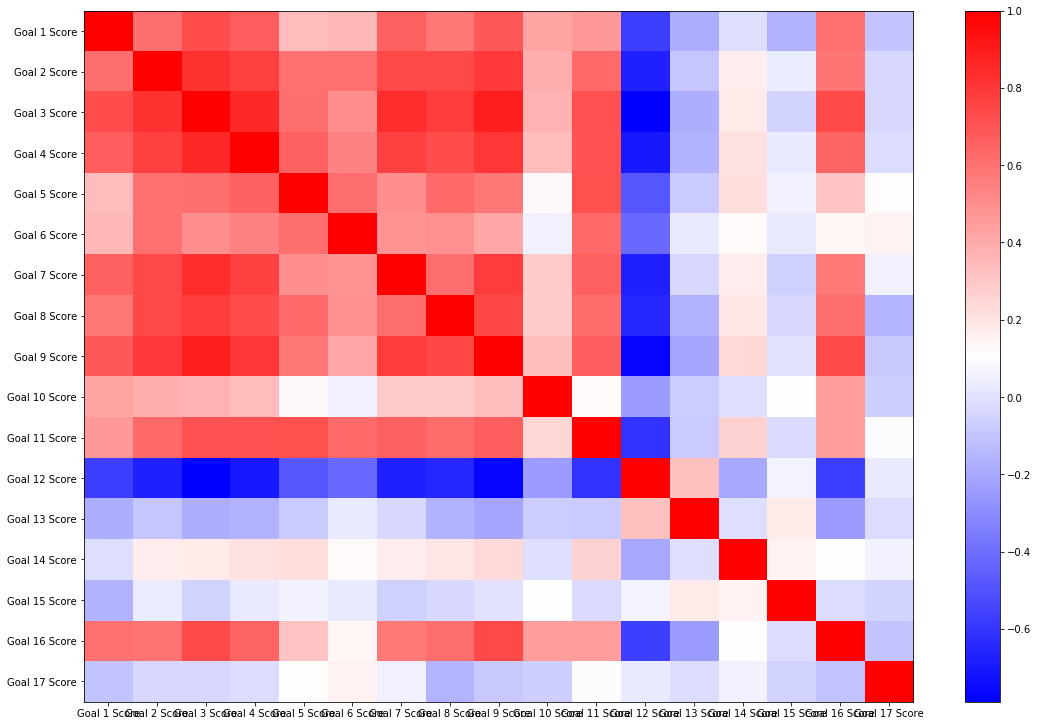
\includegraphics[width=12cm]{figures/matrix_realtion.png}
\caption{The visualization of the Adjacency matrix}
\end{figure}
% 这里多放几个图
Using the clustering approach, the adjacency matrix is divided into two components. Moreover, we establish two sets of threshold values to eliminate superfluous connections.

\section{The Model Results}
\begin{table}\caption{Statistical results}
% 这里是统计结果
\begin{center}
\begin{tabular}{p{80pt}p{80pt}p{80pt}}
\toprule
sysmtem     & Version & Editor \\
\midrule
Windows     & Mik\TeX  & \TeX{}MakerX \\
Unix/Linux  & te\TeX   & Kile \\
\bottomrule
\end{tabular}
\end{center}
\end{table}


\section{Case one: Modeling without overlap}

\subsection{Model Evaluation}%1 针对case 定义的解的评价

\subsection{Model Assumptions}%2 参数、变量、目标、模型

\subsection{Algorithm design}
\subsubsection{Multi-objective optimization algorithm}

\subsubsection{Crossover operator}

\subsection{Experiments and Analysis}%每个小节回答一个问题



\section{Case two: Modeling with overlap}
\subsection{Model Evaluation}%1 针对case 定义的解的评价

\subsection{Model Assumptions}%2 参数、变量、目标、模型

\subsection{Algorithm design}
\subsubsection{Multi-objective optimization algorithm}

\subsubsection{Crossover operator}

\subsection{Experiments and Analysis}%每个小节回答一个问题




\section{Comparative Analysis}
\subsection{ Pros and cons of the two cases}
Comparing the pros and cons of the two cases.

\subsection{Knee points selection}
\subsection{Change in priority order}




\section{Generalization}


\section{Conclusions}
\begin{itemize}
\item \textbf{Applies widely}\\
This  system can be used for many types of airplanes, and it also
solves the interference during  the procedure of the boarding
airplane,as described above we can get to the  optimization
boarding time.We also know that all the service is automate.
\item \textbf{Improve the quality of the airport service}\\
Balancing the cost of the cost and the benefit, it will bring in
more convenient  for airport and passengers.It also saves many
human resources for the airline.
\end{itemize}














% \begin{thebibliography}{99}
% \bibitem{Knuth} D.~E. Knuth.  The \TeX{}book,
% the American Mathematical Society and Addison-Wesley Publishing Company, 1984-1986.

% \bibitem{Lamport}
% Lamport, Leslie.  \LaTeX{}:``A Document Preparation System'',
% Addison-Wesley Publishing Company, 1986.

% \bibitem{latex}
% http://www.latexstudio.net/


% \bibitem{chinatex}
% http://www.chinatex.org/

% \end{thebibliography}

% \newpage
% % bibliography
\bibliographystyle{elsarticle-num}
\bibliography{sample}

%\hspace{2em}
\begin{appendices}

\section{Code of AHP}

Here are simulation programmes we used in our model as follows.\\

\textbf{\textcolor[rgb]{0.98,0.00,0.00}{Input matlab source:}}
\lstinputlisting[language=Matlab]{./code/mcmthesis-matlab1.m}

\section{Second appendix}

some more text \textcolor[rgb]{0.98,0.00,0.00}{\textbf{Input C++ source:}}
\lstinputlisting[language=C++]{./code/mcmthesis-sudoku.cpp}

\end{appendices}
\end{document}
